\documentclass{standalone}
\usepackage{tkz-fct}
\usepackage{tkz-euclide}
\usepackage{color}
\renewcommand*\familydefault{\sfdefault}
\usepackage{sansmath}
\usepackage{amsmath}
\sansmath
\definecolor{gray75}{gray}{0.75}
\begin{document}
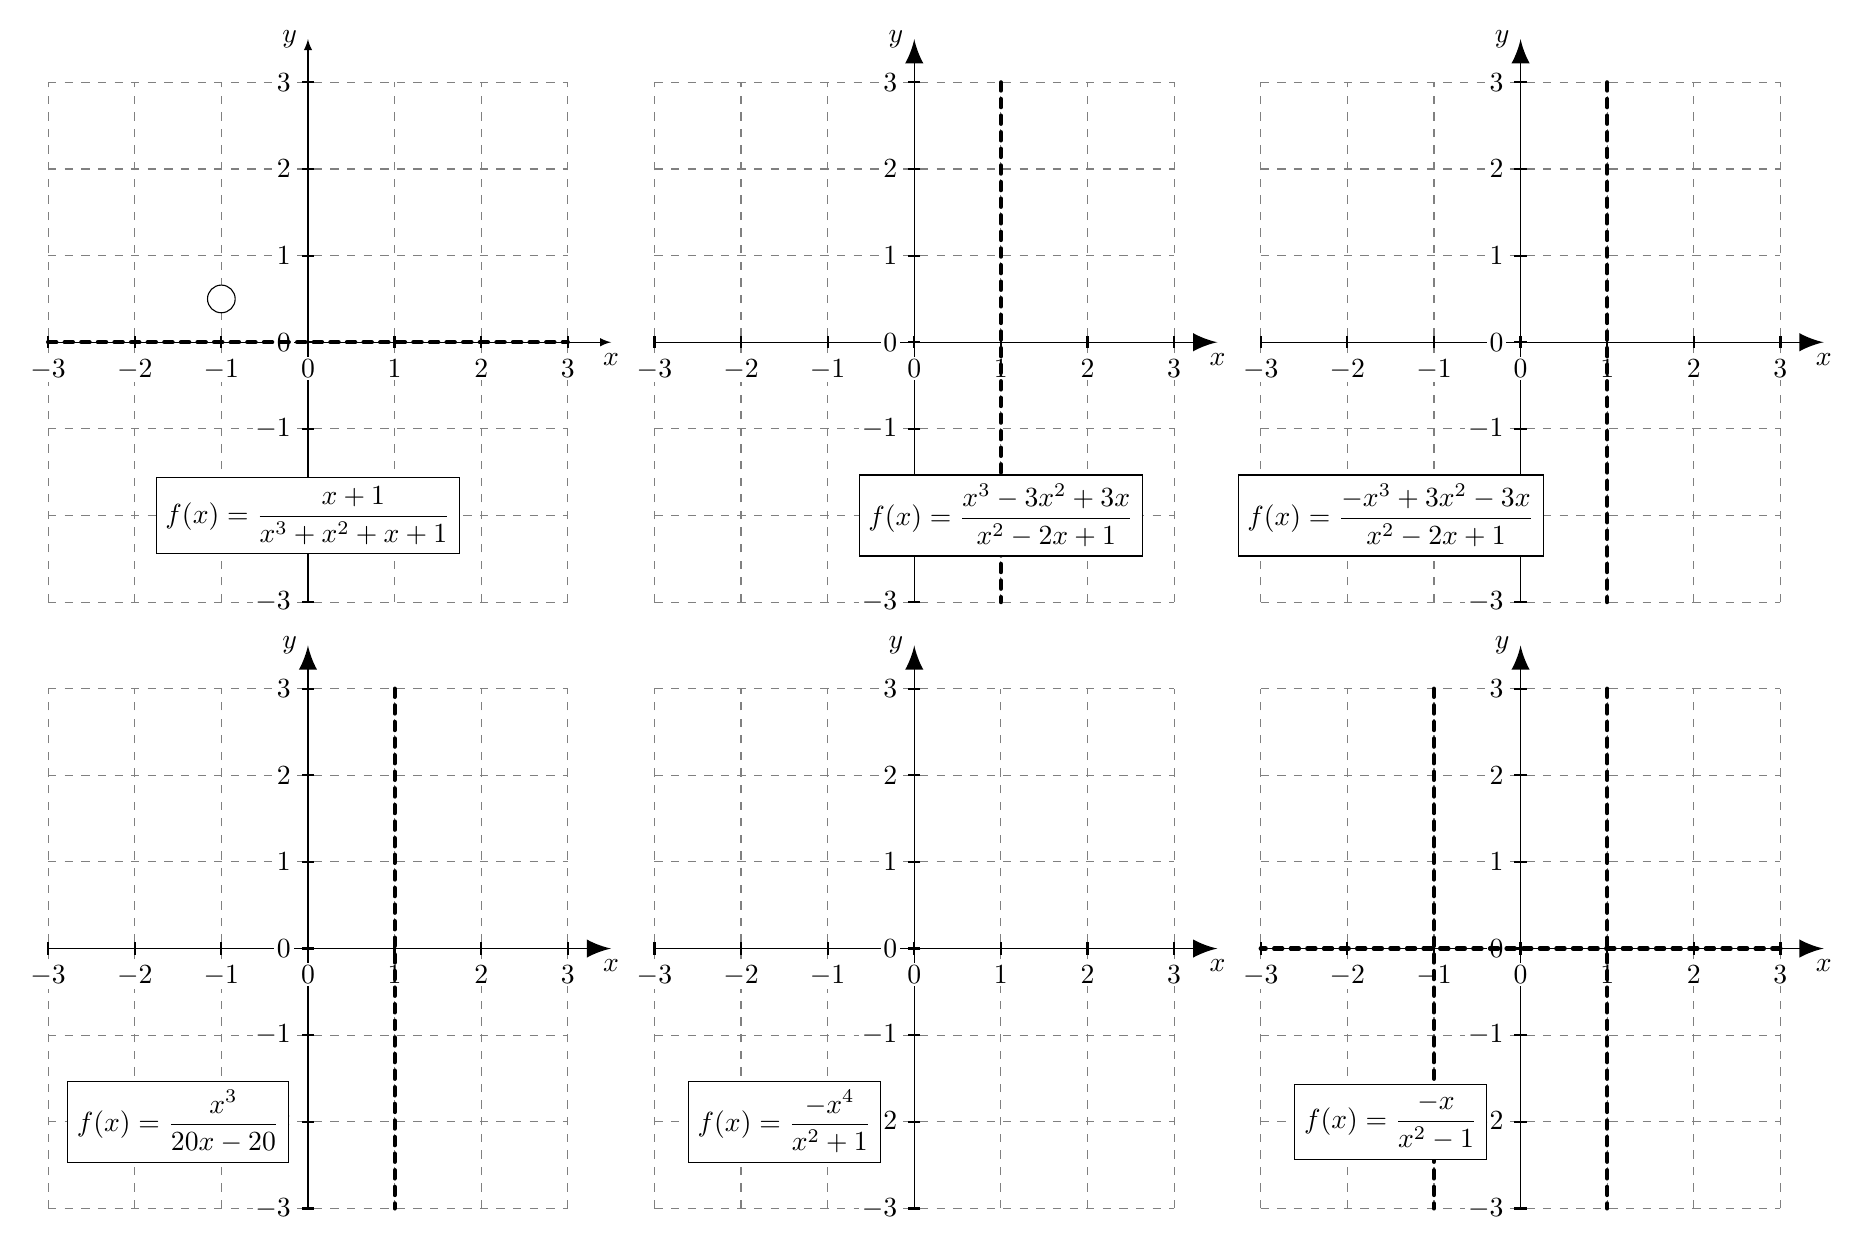
\begin{tikzpicture}[scale=1.1]
  \tkzInit[xmin=-3, xmax=3,ymin=-3,ymax=3]
  \begin{scope}[dashed]
    \tkzGrid
  \end{scope}
  \tkzDrawX[label={$x$}]
  \tkzDrawY[label={$y$}]
  \tkzLabelX
  \tkzLabelY
  \tkzFct[line width=2pt, domain=-3:3]{(x+1)/(x**3+x**2+x+1)}
  \tkzDrawPoint[size=10,color=black,fill=white](-1.0,0.5)
  \tkzDefPoint(-3.0,0){A}
  \tkzDefPoint(3.0,0){B}
  \tkzDrawSegment[style=dashed,line width = 1.5pt](A,B)
  \tkzText[draw,
  fill=white](0,-2){$f(x)=\dfrac{x+1}{x^{3}+x^{2}+x+1}$}
  \begin{scope}[xshift=7cm]
\tkzInit[xmin=-3, xmax=3,ymin=-3,ymax=3]
  \begin{scope}[dashed]
    \tkzGrid
  \end{scope}
  \tkzDrawX[label={$x$}]
  \tkzDrawY[label={$y$}]
  \tkzLabelX
  \tkzLabelY
  \tkzFct[line width=2pt, domain=-3:0.9]{x-1+1/(x-1)**2}
  \tkzFct[line width=2pt, domain=1.1:3]{x-1+1/(x-1)**2}
    \tkzFct[line width=1.5pt,dashed, domain=-3:3]{x-1}

  \tkzDefPoint(1.0,3.0){A}
  \tkzDefPoint(1.0,-3.0){B}
  \tkzDrawSegment[style=dashed,line width = 1.5pt](A,B)
  \tkzText[draw, fill=white](1,-2){$f(x)=\dfrac{x^{3}-3x^{2}+3x}{x^{2}-2x+1}$}
\end{scope}
\begin{scope}[xshift=14cm]
\tkzInit[xmin=-3, xmax=3,ymin=-3,ymax=3]
  \begin{scope}[dashed]
    \tkzGrid
  \end{scope}
  \tkzDrawX[label={$x$}]
  \tkzDrawY[label={$y$}]
  \tkzLabelX
  \tkzLabelY
  \tkzFct[line width=2pt, domain=-3:0.9]{-(x-1)-1/(x-1)**2}
  \tkzFct[line width=2pt, domain=1.1:3]{-(x-1)-1/(x-1)**2}
  \tkzFct[line width=1.5pt,dashed, domain=-3:3]{-x+1}
  \tkzDefPoint(1.0,3.0){A}
  \tkzDefPoint(1.0,-3.0){B}
  \tkzDrawSegment[style=dashed,line width = 1.5pt](A,B)
  \tkzText[draw, fill=white](-1.5,-2){$f(x)=\dfrac{-x^{3}+3x^{2}-3x}{x^{2}-2x+1}$}
\end{scope}
\begin{scope}[xshift=0cm,yshift=-7cm]
\tkzInit[xmin=-3, xmax=3,ymin=-3,ymax=3]
  \begin{scope}[dashed]
    \tkzGrid
  \end{scope}
  \tkzDrawX[label={$x$}]
  \tkzDrawY[label={$y$}]
  \tkzLabelX
  \tkzLabelY
  \tkzFct[line width=2pt, domain=-3:0.99]{x**3/(20*x-20)}
  \tkzFct[line width=2pt, domain=1.01:3]{x**3/(20*x-20)}
  \tkzDefPoint(1.0,3.0){A}
  \tkzDefPoint(1.0,-3.0){B}
  \tkzDrawSegment[style=dashed,line width = 1.5pt](A,B)
  \tkzText[draw, fill=white](-1.5,-2){$f(x)=\dfrac{x^{3}}{20x-20}$}
\end{scope}
\begin{scope}[xshift=7cm,yshift=-7cm]
\tkzInit[xmin=-3, xmax=3,ymin=-3,ymax=3]
  \begin{scope}[dashed]
    \tkzGrid
  \end{scope}
  \tkzDrawX[label={$x$}]
  \tkzDrawY[label={$y$}]
  \tkzLabelX
  \tkzLabelY
  \tkzFct[line width=2pt, domain=-3:3]{-x**4/(x**2+1)}

  \tkzText[draw, fill=white](-1.5,-2){$f(x)=\dfrac{-x^{4}}{x^{2}+1}$}
\end{scope}
\begin{scope}[xshift=14cm,yshift=-7cm]
\tkzInit[xmin=-3, xmax=3,ymin=-3,ymax=3]
  \begin{scope}[dashed]
    \tkzGrid
  \end{scope}
  \tkzDrawX[label={$x$}]
  \tkzDrawY[label={$y$}]
  \tkzLabelX
  \tkzLabelY
  \tkzFct[line width=2pt, domain=-3:-1.01]{-x/(x**2-1)}
  \tkzFct[line width=2pt, domain=-0.99:0.99]{-x/(x**2-1)}
  \tkzFct[line width=2pt, domain=1.01:3]{-x/(x**2-1)}
  \tkzDefPoint(3,0){A}
  \tkzDefPoint(-3,0){B}
  \tkzDrawSegment[style=dashed,line width = 1.5pt](A,B)
\tkzDefPoint(-1.0,3.0){A}
  \tkzDefPoint(-1.0,-3.0){B}
  \tkzDrawSegment[style=dashed,line width = 1.5pt](A,B)
  \tkzDefPoint(1.0,3.0){A}
  \tkzDefPoint(1.0,-3.0){B}
  \tkzDrawSegment[style=dashed,line width = 1.5pt](A,B)
  \tkzText[draw, fill=white](-1.5,-2){$f(x)=\dfrac{-x}{x^{2}-1}$}
\end{scope}
\end{tikzpicture}
\end{document}
